\documentclass[letterpaper,pdftex]{article}

\setlength{\textwidth}{168mm}
\setlength{\textheight}{210mm}
\setlength{\oddsidemargin}{0cm}
\setlength{\topmargin}{0cm}
\setlength{\headheight}{48pt}
\addtolength{\textheight}{-25pt}
\voffset -0.5in

\usepackage{natbib}
\usepackage[utf8]{inputenc}
\usepackage[spanish]{babel}
\usepackage{xcolor,graphicx}
\usepackage{fancyhdr}
\usepackage{multirow}
\usepackage{hyperref}
\hypersetup{
    colorlinks,
    citecolor=blue,
    filecolor=black,
    linkcolor=blue,
    urlcolor=black
}
\usepackage{epstopdf}
\usepackage[autolinebreaks,useliterate]{mcode}
\pagestyle{fancy}
\renewcommand{\headrule}{\color{gray}
\hrule width\headwidth height\headrulewidth \vskip-\headrulewidth}
\renewcommand{\footrule}{{\color{gray}
\vskip-\footruleskip\vskip-\footrulewidth
\hrule width\headwidth height\footrulewidth\vskip\footruleskip}}
\renewcommand{\headrulewidth}{1.5pt}
\renewcommand{\footrulewidth}{1.5pt}

\spanishdecimal{.}

\begin{document}
\fancyhead{}
\fancyfoot{}
\fancyhead[L]{
\begin{minipage}{3.5cm}
\begin{center}
	
\includegraphics[width=0.95\textwidth]{logousb.png}
\end{center}
\end{minipage}
\begin{minipage}{12cm}
\begin{flushleft}
\small \textsc{Universidad de San Buenaventura}\\
\small \textsc{Facultad de Ingeniería}\\
\small \textsc{Programa de Ingeniería Mecatrónica\\}
\end{flushleft}
\end{minipage}
}
\fancyhead[R]{
\begin{minipage}{3.0cm}
\begin{flushright}
\small \textsc{Dibujo de \\ Máquinas}\\
\small \textsc{2021-I}
\end{flushright}
\end{minipage}
}
\fancyfoot[R]{\large \textbf{\thepage}}

\begin{minipage}{0.3\textwidth}
\begin{flushleft}
\textbf{Autor:}\\
\textit{Nikolay Prieto Ph.D(c)}\\
\end{flushleft}
\end{minipage}
\begin{minipage}{0.7cm}
\textcolor{gray}{\rule{0.3cm}{2.5cm}}
\end{minipage}
\begin{minipage}{0.64\textwidth}
\Large{\textbf{Procedimiento Proyecto \\ Dibujo de Máquinas \\ Dimesionamiento (Parte I)}}
\end{minipage}\\

\noindent
\textcolor{gray}{\rule{\textwidth}{0.5pt}}\\
\renewcommand{\tablename}{Tabla}
\renewcommand{\arraystretch}{1.2}
\renewcommand\contentsname{Contenido}
\tableofcontents

\noindent
\textcolor{gray}{\rule{\textwidth}{0.5pt}}\\

\section{Introducci\'on}

El objetivo del presente es mostrar a los estudiantes el procedimiento del proyecto final, referente al Dibujo de Máquinas (DM). Esta actividad pretende fortalecer las siguientes competencias, modificadas acorde a lo propuesto por \cite{Metraglia2014}:

\begin{itemize}
\item Interpretar la morfología de un sólido, a raíz de la representación en vistas y secciones.
\item Desarrollar capacidad en la medición de precisión con partes mecánicas.
\item Proponer independientemente la representación óptima de una pieza a través de vistas y secciones. 
\item Implementar las buenas prácticas de dimensionamiento mencionadas en la NTC1960 \cite{ICONTEC2009}
\item Reconocer las formas roscadas y representarlas acorde al estándar itnernacional.
\item Implementar ajustes y tolerancias entre partes interconectadas.
\item Tener el criterio en la implementación de tolerancias geométricas.
\item Tener en cuenta la incertudumbre en la precisión del mecanizado con el fin de proponer un ajuste dimensional a través de tolerancias dimensionales.
\end{itemize} 

Organice esta actividad con un compañero del curso, la idea es seleccionar un objeto físico desarmable, medible y que contenga las siguientes características mecánicas. Los requisitos son los siguientes:

\begin{enumerate}
\item Insertos cilíndricos y de otra otra geometría: Elementos que encajen con otros bien sea a presión, justo o deslizante. El objetivo es que configuren el tipo de ajuste en el plano. Ejemplos de ello son los empaques de caucho de las licuadoras, los mangos de las bicicletas, entre otros.
\item Por cada integrante del grupo son mínimo 10 piezas, es decir, si su grupo es de 2, debe presentar un conjunto de 20 piezas mínimo. De trabajar individualmente, serían 10.
\item El mecanismo debe tener piezas movibles. El objetivo es que ustedes reproduzcan en el CAD los movimientos cinemáticos del artefacto a replicar.
\item Deben comprar calibrador de Vernier, aunque es recomendable comprar uno metálico, con el de plástico (que es más económico) pueden realizar el ejercicio.
		
\item El mecanismo debe contener mínimo 2 tipos de piezas entre los sigueintes elementos:

	\begin{itemize}
	\item Elementos roscados: Pernos, tuercas y tornillos.
	\item Resortes de cualquier índole.
	\item Rodamientos 
	\item Cadenas
	\item Levas.
	\item Engranajes.
	\end{itemize}
	

\end{enumerate}

El proyecto es mención debe ser aprobado en principio para determinar si cumple con las condiciones. Diligencie la siguiente hoja de excel \href{https://usbbogedu-my.sharepoint.com/:x:/g/personal/eprieto_usbbog_edu_co/EbDnMvzuUtpPljIkT-3NsnMBCzidd8gOxdZgFu1oSlNxJw?e=AHxVcA}{Click acá} en la cual encontrará distintos ejemplos de proyectos que se pueden realizar en casa.

Para cumplir con lo anterior se presentan 4 grandes actividades cuya explicación se divide en las siguientes secciones.

\begin{itemize}
\item Dimensionamiento. (27/05/2021).
\item Modelo CAD (27/05/2021).
\item Simulación de movimiento (Cinemática) y validación de esfuerzos (3/06/2021).
\item Representación en planos (3/06/2021).
\end{itemize}

Este documento trata la primera sección y parte de la segunda.

\section{Dimensionamiento}

Para el dimensionamiento debe realizar el siguiente proceso, bien sea con el calibrador de Vernier o micrómetro:

\begin{enumerate}
\item Verifique que no tenga error de cero el elemento. De lo contrario tendrá que restar o sumar ese error.
\item Utilice la geometría del calibrador de vernier indicada para cada elemento. Ejemplo, si va a medir profundidad use la barra; las mordazas para exteriores son para elementos como su nombre lo indica: superficies; para medir agujeros use las mordazas interiores. 
\item Para los elementos cilíndricos tome mínimo 4 dimensiones alrededor del cilindro, ejemplo: 0°, 90°, 270° y 360°.
\item Para elementos planos realice mínimo tres dimensiones en diferentes lugares de cada cara.
\item Tome solo las medidas necesarias y registrélas en una tabla de excel, un ejemplo se muestra en la tabla \ref{tab:muestra}. De ese ejemplo, la cota queda de $10.445 \pm 0.1477$
\item Tome tres cifras de precisión después de la décima.
\item Maneje solamente milímetros o pulgadas como unidad de medida.

\begin{table}
\begin{centering}
\begin{tabular}{|c|c|c|c|}
\hline 
\multicolumn{4}{|c|}{Parte 1 (agujero X)}\tabularnewline
\hline 
No. muestra & Dimensión & media & STD\tabularnewline
\hline 
\hline 
1 & 10.25 & \multirow{4}{*}{10.445} & \multirow{4}{*}{0.1477}\tabularnewline
\cline{1-2} \cline{2-2} 
2 & 10.38 &  & \tabularnewline
\cline{1-2} \cline{2-2} 
3 & 10.5 &  & \tabularnewline
\cline{1-2} \cline{2-2} 
4 & 10.65 &  & \tabularnewline
\hline 
\end{tabular}
\par\end{centering}
\caption{Tabla de indicación dimensional. (Ejemplo)}
\label{tab:muestra}
\end{table}
\end{enumerate}

\begin{figure}
\begin{center}
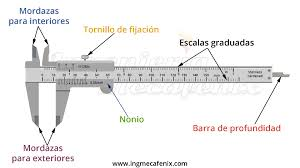
\includegraphics[scale=0.7]{calibrador.jpeg}
\caption{Partes de un calibrador.}
\label{fig:calibrador}
\end{center}
\end{figure}

\section{Forma de entrega}

Un informe en el editor documental de su preferencia, bien sea en word o Latex. En donde se especifique el sketch (ver fig. \ref{fig:sketch}) de cada pieza, señalando la parte y la posición que indica la medida. A su vez, se deben mostrar las tablas para cada dimensión, tal como se indica en \ref{tab:muestra}. El informe debe mostrar los siguientes aspectos:

\begin{itemize}
\item Mencione el procedimiento que realizó. Ubique un espacio óptimo de trabajo, buena iluminación, espacio limpio, entre otras cosas relevantes que usted usó para el proceso de medición.
\item Enuncie el listado de piezas completo, partes repetidas cuentan como una sola pieza.
\item Pantallazos de los sketch del conjunto.
\item Incluya al menos 1 foto legible para cada caso de dimensionamiento (profundidad, exteriores e interiores). Para la foto debe poderse leer la medida. Ejemplo mostrado en la Fig. \ref{fig:medida}
\item Coloque las tablas para cada geometría a tomar dimensión.
\item Realice conclusiones acerca del trabajo que realizó.
\item Fecha de entrega: 
\begin{itemize}
\item \textbf{Dimensionamiento y Modelos CAD:} 27/05/2021
\item \textbf{Render, simulación cinemática y entrega de planos:} 3/06/2021 
\end{itemize}
\end{itemize}

\begin{figure}
\begin{center}
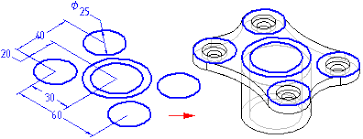
\includegraphics[scale=0.7]{sketch.png}
\caption{Sketch de la pieza a dimensionar. De este ejemplo deben haber 5 tablas que establezcan la medida.}
\label{fig:sketch}
\end{center}
\end{figure}

\begin{figure}
\begin{center}
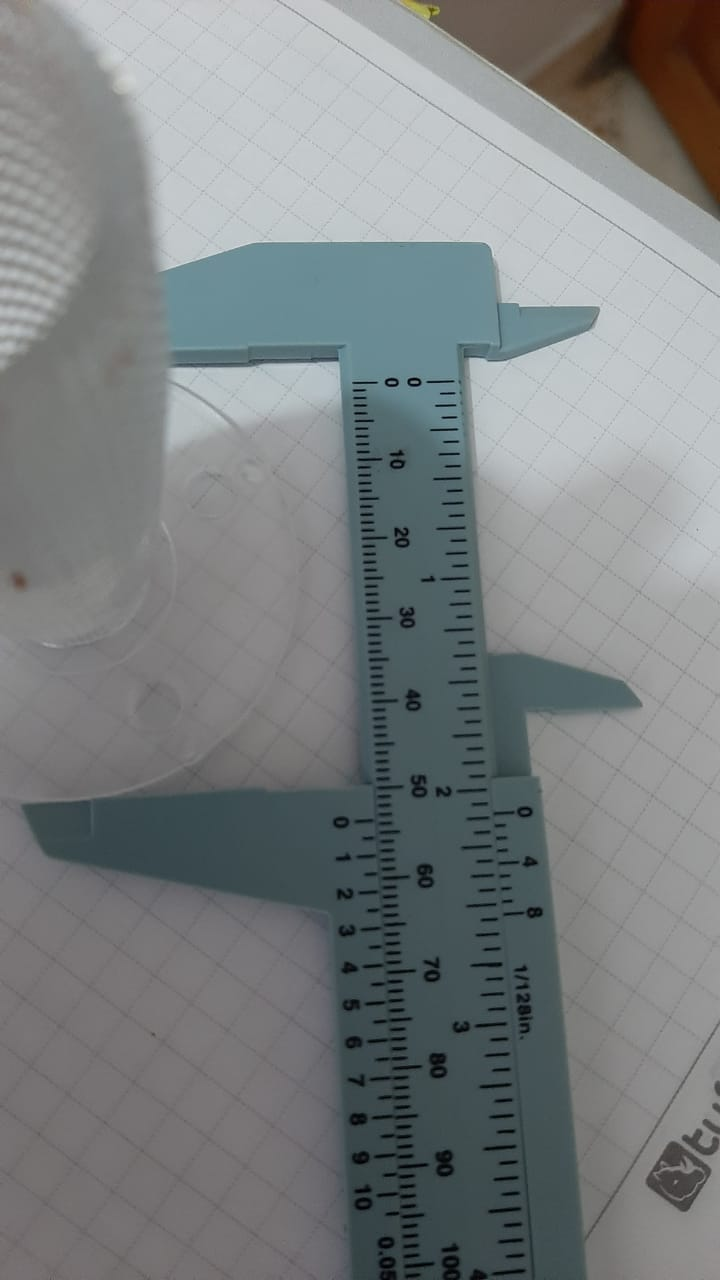
\includegraphics[scale=0.2]{medida}
\caption{Ejemplo de una muestra dimensional para exteriores.}
\label{fig:medida}
\end{center}
\end{figure}

\bibliography{Referencias}
\bibliographystyle{apalike} %apalike


\end{document}
